\documentclass[a4paper, 10pt]{report}
\usepackage[italian]{babel}
\usepackage[T1]{fontenc}
\usepackage[utf8]{inputenc}
\usepackage{charter}
\usepackage{amsmath}
\usepackage{amsthm}
\usepackage{amsfonts}
\usepackage{graphicx}
\usepackage{wrapfig}
\usepackage{tcolorbox}
\usepackage{fancyhdr}
\usepackage{longtable}

\usepackage{geometry}
\geometry{a4paper, left=2cm,right=2cm,top=2cm,bottom=2cm}

\pagestyle{fancy}
\chead{}
\rhead{\bfseries 22 ottobre 2019}
\lhead{\bfseries Basi di dati}

\begin{document}
\noindent La rappresentazione binaria della precedente ternaria può essere la seguente: 

\begin{center}
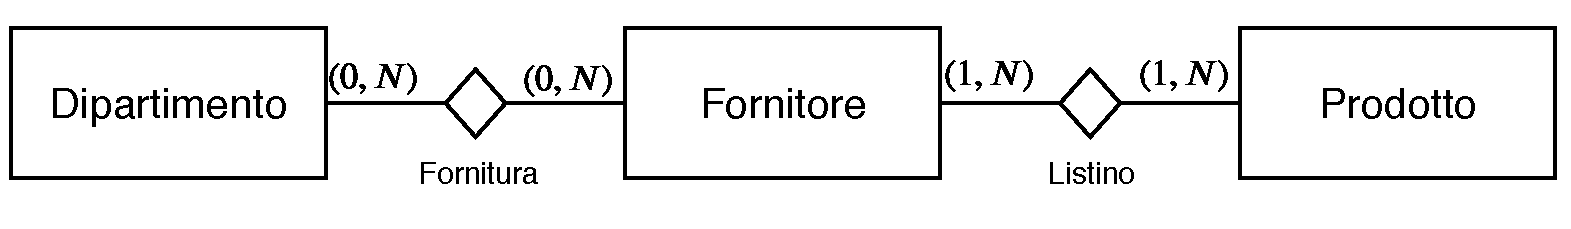
\includegraphics[scale=0.5]{22ottobre01.pdf}
\end{center}

\noindent L'informazione che vado a rappresentare in questo modo, però, differisce da quella rappresentaata attraverso la relazione ternaria. Infatti:

\begin{longtable}{ p{.30\textwidth} p{.30\textwidth} p{.30\textwidth}}

I(fornitura) = \{

(d1, f1), 

(d1, f3), 

(d2, f1), 

(d2, f2)

\} & I(listino) = \{

(f1, p1), 

(f1, p3), 

(f3, p3), 

(f3, p2)

\} & I(composizione) = \{

(d1, f1, p1), 

(d1, f1, p3), 

(d1, f3, p3), 

(d1, f3, p2), 

...
\}
\end{longtable}

\noindent Con due relazioni binarie, quindi, vado a rappresentare più combinazioni rispetto alla ternaria. La trasformazione di una relazione da ternaria a doppia binaria dipende dalla situazione. In ogni caso, per poter fare ciò, una delle entità che partecipa alla relazione ternaria deve avere cardinalità $(1, 1)$.\\

\noindent Gli errori principali nell'uso delle relazioni ternarie si hanno quando:
\begin{itemize}
\item[-] Per rappresentare un'istanza del concetto che ho modellato con una ternaria ho bisogno solo di una coppia di istanze di entità (manca un'istanza alla terna);
\item[-] Per rappresentare un'istanza del concetto che ho modellato con una ternaria devo aggiungere più terne ridondanti.  
\end{itemize}

\paragraph*{Storicizzazione} Si può utilizzare una relazione ternaria per storicizzare relazioni binarie:

\begin{center}
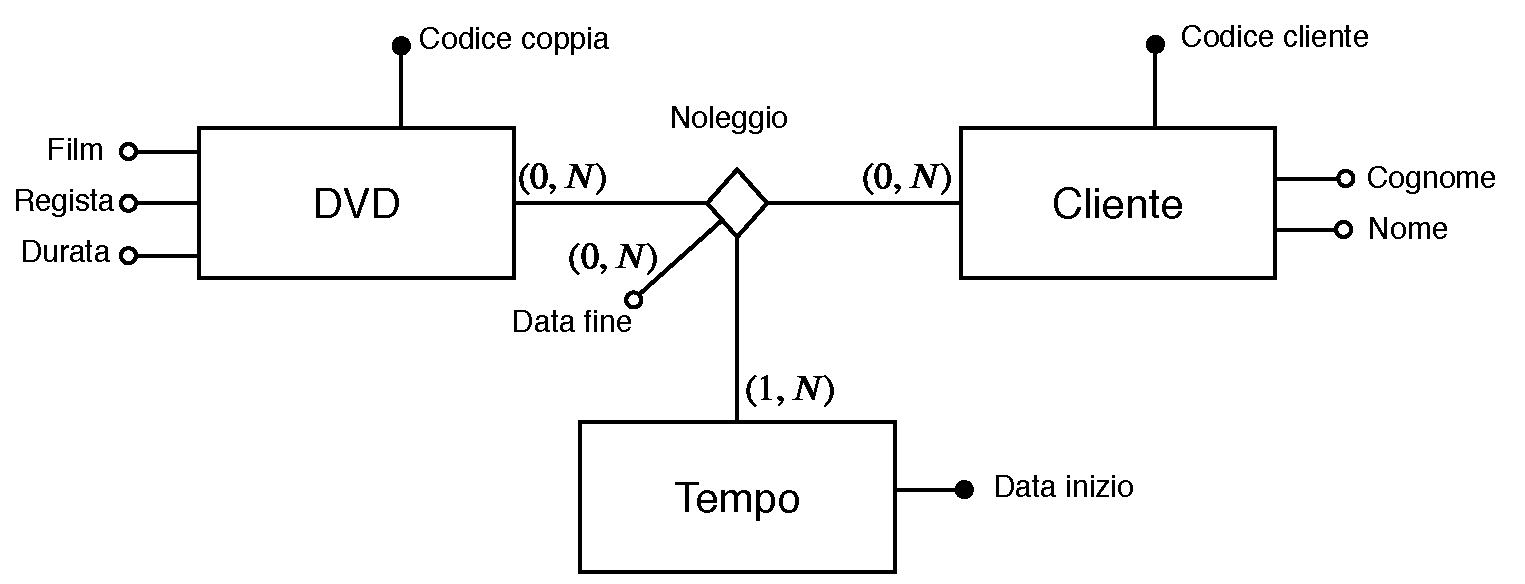
\includegraphics[scale=0.5]{22ottobre02.pdf}

(data\_inizio deve essere identificatore e data\_fine deve essere attributo della relazione)
\end{center}



\noindent ATTENZIONE: è sempre possibile trasformare una relazione ternaria in un'entità.
\end{document}